



\begin{myact}{3}
	Activité 2 page 12
\end{myact}


\begin{myactrep}{2 page 12}
	\begin{enumerate}
		\item Je convertis les fractions en nombre décimal :
		
		$ \dfrac{3}{100} = 3 \div 100 = \num{0.03}$ ; $\dfrac{91}{100} = 91 \div 100 = \num{0.91}$; $\dfrac{956}{100} = 956 \div 100 = \num{9.56}$; $\dfrac{18}{1000} = 18 \div 1000 = \num{0.018}$
		
		J'additionne ces nombres aux temps et j'obtiens :
		
		\begin{tabular}{|@{\ }c@{\ }|@{\ }c@{\ }|@{\ }c@{\ }|@{\ }c@{\ }|@{\ }c@{\ }|@{\ }c@{\ }|@{\ }c@{\ }|@{\ }c@{\ }|@{\ }c@{\ }|}
			\hline
			Appel à      & Léa         & Chloé       & Djamila      & Sarah        & Marine      & Sophiane    & Cindy        & Charlotte    \\ \hline
			Temps (en s) & \num{19.98} & \num{20.03} & \num{29.690} & \num{19.893} & \num{19.91} & \num{28.56} & \num{20.018} & \num{19.935} \\ \hline
		\end{tabular}
		
		C'est donc avec Djamila qu'elle a passé le plus de temps et avec Sarah le moins.
		
		\item Je classe les appels téléphoniques du plus court au plus long :
		
		Sarah, Marine, Charlotte, Léa, Cindy, Chloé, Sophiane, Djamila.
	\end{enumerate}
\end{myactrep}

\begin{mydef}
	\begin{itemize}
		\item Une \kw{fraction}, notée $\dfrac{n}{d}$ est une division entre deux nombres $n$ et $d$, séparés par un trait de fraction.
		
		\item $n$ est le \kw{numérateur} , $d$ est le \kw{dénominateur}.
	\end{itemize}

	
	
\end{mydef}

\begin{myex}
	$\dfrac{15}{5}$ est une fraction.
	
	\begin{center}
		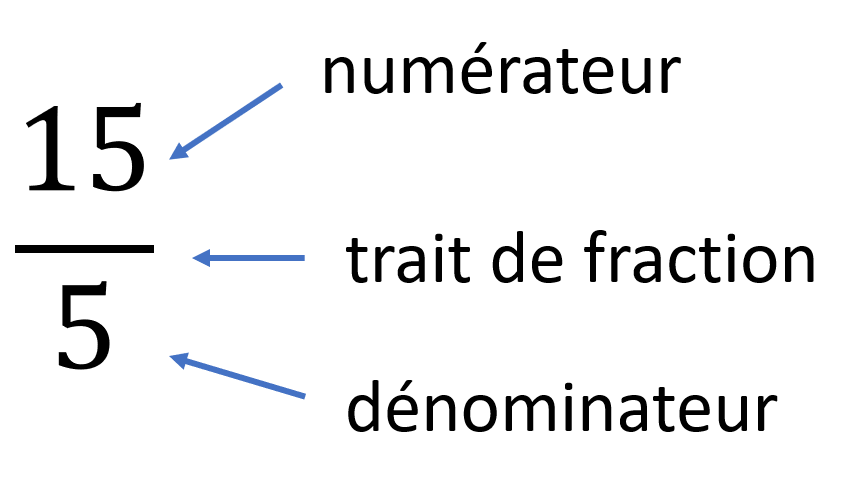
\includegraphics[scale=0.4]{img/frac2}
	\end{center}
\end{myex}

\begin{mydef}
	\begin{itemize}
		\item Une \kw{fraction décimale}, est une fraction où le dénominateur est un multiple de 10.		
		
		\item Toute fraction décimale peut s'écrire sous la forme d'un nombre décimal. C'est son \kw{écriture décimale}.
	\end{itemize}	
	
\end{mydef}


\begin{myexs}
	\begin{itemize}
		\item $\dfrac{145}{10}$ est une fraction décimale, son écriture décimale est \num{14.5}.
		\item $\dfrac{72}{100}$ est une fraction décimale, son écriture décimale est \num{0.72}.
		\item $\dfrac{9}{1000}$ est une fraction décimale, son écriture décimale est \num{0.009}.
	\end{itemize}
\end{myexs}

